\section{Software Maintainability} \label{chapter3:software-maintainability}

\cit{It is becoming increasingly important to the data-processing industry to be able to produce more programming systems and produce them with fewer errors, at a faster rate, and in a way that modifications can be accomplished easily and quickly.}{W. P. Stevens, G. J. Myers, L. L. Constantine \cite{Stevens1974}}.

In order to improve and maintain a software system, it is important to holds in mind the mental representation behind its implementation.
Architects, and mechanical engineers draw codified plans to share their mental representations with peers and building teams.
software design is an exception in that the implementation is both the shared mental representation, and the actual product.
The mental representation is often lost in technical details and optimizations for the actual product.
This problem becomes even more critical as the system grows in size.
Therefore, it is crucial to decompose the system into smaller subsystem easier to grasp individually.
This section shows the theories, programming languages and frameworks helping this decomposition.

\subsection{Modular Programming} \label{chapter3:software-maintainability:modular-programming}

The modularity of a software implementation is about enclosing the subproblems and bringing the relevant interfaces to allow these part to be composed.
It allows greater design to emerge from the composition of smaller components.
Such modularity helps organizing the implementation to reflect the underlying mental organization.
The modularity in software design improves the maintainability of an implementation, as presented in the following schema.
It allows to limit the understanding required to contribute to a module \cite{Stevens1974}.
And it reduces development time by allowing several developers to simultaneously implement different modules \cite{Wong2009,Cataldo2006}.

\begin{center}
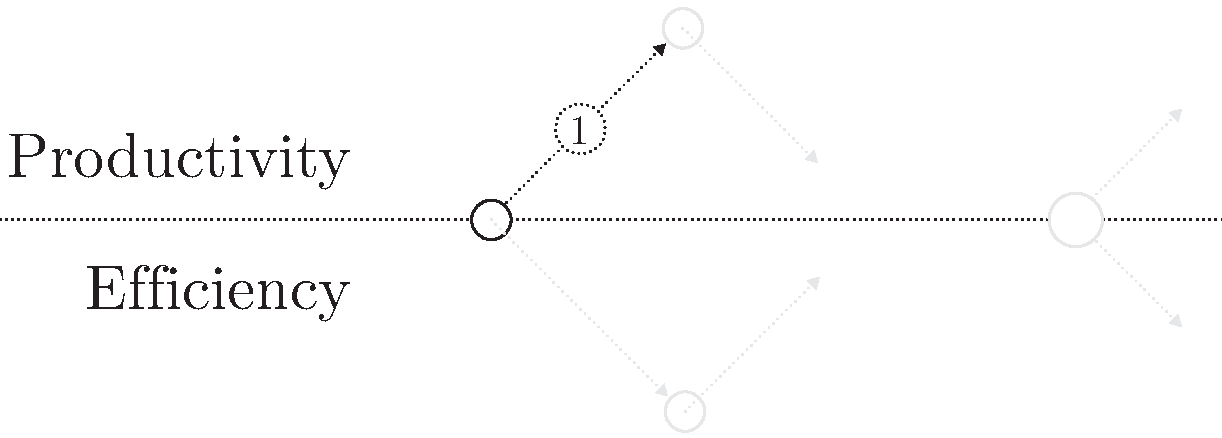
\includegraphics[width=0.6\textwidth]{../ressources/state-of-the-art-1.pdf}
\end{center}

The section \ref{chapter3:software-maintainability:modular-programming:design-choices} is about the decomposition of a problem into subproblems.
Then, the section \ref{chapter3:software-maintainability:modular-programming:programming-models} is about the bringing the interfaces allowing their composition.
Finally, the section \ref{chapter3:software-maintainability:modular-programming:limitations} presents the consequences of this decomposition on performance.


\subsubsection{Design Choices} \label{chapter3:software-maintainability:modular-programming:design-choices}

\nt{TODO this introduction is not very clear}
In the decomposition of a large problem into smaller subproblem, there is two design choices.
The first one is the granularity, and organization of the subproblems within the system decomposition.
The second one is the organization of the implementation within the subproblems to improve maintainability.

\paragraph{System Decomposition}

\illustration{spaghetti programming}

Dijkstra firstly developed the concept of Structured Programming \cite{Dijkstra1970}, which later led to modular programming.
% It is defined as \textit{the systematic use of abstraction to control a mass of details, and also a means of documentation which aids program design} \cite{Knuth1974}.
Structured programming is about drawing clear interfaces around a piece of implementation so that the execution is clearly enclosed inside.
At a fine level, it helps avoid spaghetti code \cite{Dijkstra1968a}, and at a coarser level, it structures the implementation \cite{Dijkstra1968} into modules, or layers.
The next paragraph explains further the criteria to draw the borders around modules.

\illustration{lasagna programming}

\paragraph{Decomposition Criteria}

\nt{move this paragraph closer to OOP ?}
The criteria to decompose the system into well defined modules are coupling and cohesion \cite{Stevens1974}.
The coupling defines the strength of the interdependence between modules, while cohesion defines how strongly the features inside a module are related.
Low coupling between modules and high cohesion inside modules helps logically organize, and understand the implementation.
Hence, it improve its maintainability.
The next paragraph present the approach to build modules helping with the evolution of the implementation.

\paragraph{Development Evolution}

To improve maintainability of implementation, the modular organization should isolate the evolution of a module from impacting the rest of the implementation.
The Information Hiding Principle \cite{Parnas1972}, and the Separation of Concerns \cite{Tarr1999,Hursch1995} are two similar approach to do so.
The information hiding principle advocates to encapsulate a specific design choice in each module.
The Separation of Concerns advocates each module to be responsible for one and only one specific concern.
Examples of separation of concerns are the separation of the form and the content in HTML / CSS, or the OSI model for the network stack.

\subsubsection{Programming Models} \label{chapter3:software-maintainability:programming-models}

The previous section presented the design choices to build modules.
This section presents the programming models providing the interfaces to glue the modules together.
It focus on two main programming models currently used in the industry, object oriented programming and functional programming.

\paragraph{Object Oriented Programming}

\illustration{multiple cells communicating}

Alan Kay, who coined the term, states that Object Oriented Programming (OOP) is about message-passing, encapsulation and late binding.
(There is no academic reference for that, only a public mail exchange\ftnt{http://userpage.fu-berlin.de/~ram/pub/pub\_jf47ht81Ht/doc\_kay\_oop\_en}.)
Message-passing and late binding loosen coupling between objects, while encapsulation is intended to increase cohesion \ftnt{http://williamdurand.fr/2013/06/03/object-calisthenics/}.
% Reducing coupling and increasing cohesion are further sought by object calisthenics, in the chapter 6 of \textit{The Thoughtworks Anthology} \cite{Bay2008}

The very first OOP language was Smalltalk \cite{Goldberg1984}.
It defined the core concept of OOP.
Nowadays, the major emblematic figures of OOP in the software industry are C++ and Java \cite{Gosling2000,Stroustrup1986}.
Though, the trend seems to digress from these languages to evolve toward a more dynamic approach, closer to Functional Programming.
Indeed Javascript adopts some functional features such as dynamic typing and higher-order functions \cite{Ecma1999}.

\paragraph{Functional Programming} \label{chapter3:software-maintainability:programming-models:functional-programming}

% \cit{All problems in computer science can be solved by another level of indirection}{Butler Lampson}

The definition of pure Functional Programming resides in manipulating only mathematical expressions - functions - and forbidding state mutability.
The absence of state mutability makes a function referentially transparent, and thus side-effect free.
The most important pure Functional Programming languages are Scheme \cite{Rees1986}, Miranda \cite{Turner1986}, Haskell \cite{Hudak1992}, Erlang \cite{JoeArmstrong} and Standard ML \cite{Milner1997}.

\nt{TODO find a better argument to say that immutability is unadapted to every day programming}
However, the functional programming concepts are also implemented in other languages along with mutable states.
Major imperative programming languages now commonly present higher-order functions and lazy evaluation to help loosen the couple between modules, define more generic and reusable modules.
\textit{In fine}, it helps developers to write applications that are more maintainable, and favorable to evolution \cite{Hughes1989,Turner1981}.

\paragraph{Higher-Order Programming}
\nt{If possible, include this reference : Continuations and coroutines \cite{Haynes1984}}

Higher-order programming allows to manipulate functions like any other primary value : to store them in variables, or to pass them as arguments.
It replaces the need for most modern object oriented programming design patterns \ftnt{http://stackoverflow.com/a/5797892/933670}.
For example Inversion of Control \cite{Johnson}, the Hollywood Principle \cite{Sweet1985}, and Monads \cite{Wadler1992}.
Higher-order programming help loosen coupling, thus improve maintainability.

In languages allowing mutable state, higher-order functions are implemented as closure, to preserve the lexical scope \cite{Sussman1998}.
A closure is the association of a function and a reference to the lexical context from its creation.
It allows this function to access variable from this context, even when invoked outside the scope of this context.
It eventually tangles the memory references so that it requires a global memory.

\paragraph{Lazy Evaluation}

Lazy evaluation is an evaluation strategy allowing to defer the execution of a function only when its result is needed.
% And according to \cite{Hughes1989}, \textit{Abelson and Sussman stress that streams (lazy list) is a powerful tool for structuring programs \cite{Sussman1983}.
The lazy evaluation of lists is equivalent to a stream with a null-sized buffer, while the opposite, eager evaluation, corresponds to an infinite buffer \cite{VanRoy2003}.
Indeed, the dataflow programming paradigm resulting from lazy lists is particularly adapted for stream processing applications.

The lazy evaluation, as well as streams are powerful tools for structuring modular programs \cite{Sussman1983}.s
Lazy evaluation allows the execution to be organized as a concurrent pipeline, as the stages are executed independently for each element of the stream.
But this concurrency requires immutability of state, or at least isolation of side-effects.
The next section addresses the consequences of higher-order programming and lazy evaluation on parallelism.

% Pipeline parallelism is relevant for multi-pass algorithms \cite{Conway1963}, and it is particularly efficient for stream processing applications.

\subsubsection{Performance Limitations} \label{chapter3:software-maintainability:modular-programming:limitations}

Functional programming greatly support modularity to improve the maintainability of an application, and its resilience to evolution.
However, the closures introduced by higher-order programming require to share the execution context among modules.
The previous chapter show that sharing makes parallelism difficult.
It is the reason why that maintainability and performance seem hardly compatible.
This section explore in further details the limitation of modular programming regarding performances.

\paragraph{Tighten Memory}

Closures are implemented in languages using a global memory.
And by exchanging closures, two modules intricately share their contexts of execution.
Higher-order programming loosen the couple on the implementation level of the modules, but tighten it on the execution level.
It improves modularity, but it inherently worsens the parallelization hence the performance scalability.

\paragraph{Scalability Limitations}

\cit{No matter how great the talent or efforts, some things just take time. You can't produce a baby in one month by getting nine women pregnant.}
{Warren Buffett\ftnt{http://www.goodreads.com/quotes/476827-no-matter-how-great-the-talent-or-efforts-some-things}}

Parallelizing the execution increases the performances \cite{Amdahl1967,Gunther1993}
But the parallelism is limited because the execution portions sharing state need to be scheduled sequentially.
Hence, to increase the parallelism and performance, the concurrent executions need to be independent, or to coordinate to be scheduled sequentially \cite{Gustafson1988,Gunther1996,Nelson1996,Gunther2002}.
We explain further the reasons of these limitations, and the improvement solutions in the next section.

\paragraph{}


\begin{table}
\small
\begin{tabu} to \linewidth {@{} *1{X[c]} | *2{X[c]} | *3{X[c]} @{}}
%
\toprule
\multicolumn{3}{c}{} & \multicolumn{3}{|c}{Modularity} \\
& Model & Examples     & Higher-Order Programming & Closures & Lazy Evaluation / Streams \\
\midrule
% ✖ ⨯ ✔                                                                       HOP  CLS  LZY 
\multirow{2}{*}{\begin{sideways}\parbox{2.3cm}{Modular Programming}\end{sideways}} & %
  Object-Oriented Programming           & C/C++, Java                       & \V & \X & \X \\
& Functional Programming                & Javascript                        & \V & \V & \V \\
\bottomrule
\end{tabu}
\caption{Synthesis of the state of the art in modular programming}
\end{table}




\nt{TODO the transition is not very clear}
The modular organization of implementation is opposed to the organization favoring the parallelization of the execution.
The former organization supports the development scalability, while the latter supports performance scalability.
A program cannot trivially follow an organization that support both development evolution, and performance.
However, D. Parnas advocates the use of an assembler to conciliate the two approaches \cite{Parnas1972}.
The next section shows the improvements for performance and parallelism .
Then, section \ref{chapter3:software-performance} shows the techniques for parallelism.

\subsection{Performance Improvements} \label{chapter3:software-maintainability:performance}

To assure its integrity, the global state of an application imposes the concurrent executions to coordinate their accesses.
This coordination is responsible of the atomicity, and exclusivity of the accesses.
It assures the invariance of the state during its atomic manipulation.
So that developers can group operations in atomic manipulations so as to avoid corruption of the state.

The invariance is assured differently depending on how the state is shared among the concurrent execution.
To increase performance, concurrent executions needs to be as independent as possible to be executed in parallel \ftnt{http://joeduffyblog.com/2010/07/11/thoughts-on-immutability-and-concurrency/}.
% Isolation is independent processes
% Immutability Immutability
% Synchronization is event-loop, multi-thread, lock-free
\begin{description}
  \item[Isolation] If different concurrent executions are commutative \cite{Rinard1996,Clements2013a}, and they share no portion of the state and can be isolated and executed in parallel.
  \item[Immutability] Otherwise, the sharing state portions needs to be immutable to conserve invariance and parallel execution \cite{Gordon2012,Matsakis2012a}.
  \item[Synchronization] If different concurrent executions needs mutation on the state, their accesses are scheduled sequentially.
\end{description}

\begin{center}
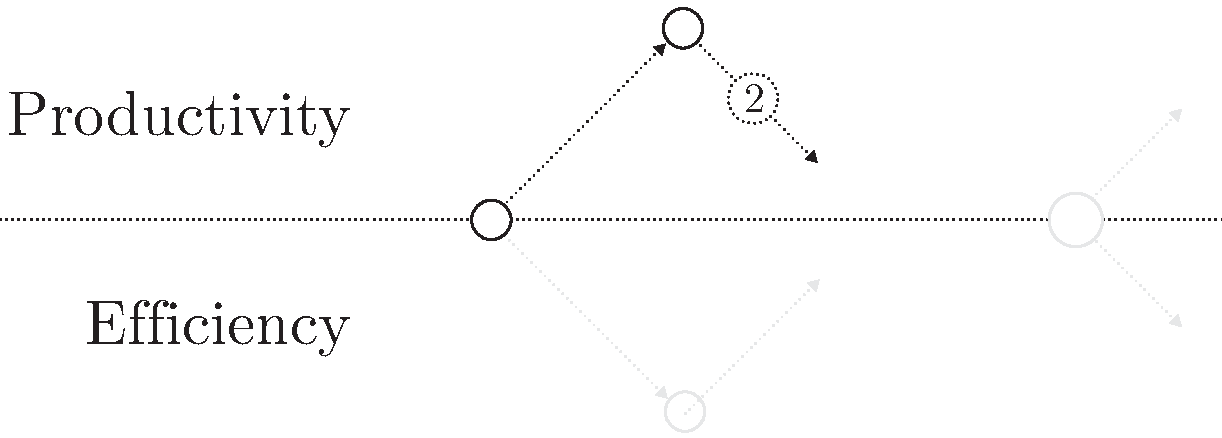
\includegraphics[width=0.6\textwidth]{../ressources/state-of-the-art-2.pdf}
\end{center}

The next few paragraphs presents the different models to assure invariance in concurrent execution, while conserving modular programming, as illustrated in the schema above.
Section \ref{chapter3:software-maintainability:performance:concurrent-programming} presents the programming models providing synchronization and immutability for concurrent executions.
Section \ref{chapter3:software-maintainability:performance:compilation} presents compilation methods to parallelize sequential programs.

% Dynamic Isolation + Making asynchronous parallelism safe for the world \cite{Jr1990}

\subsubsection{Concurrent Programming} \label{chapter3:software-maintainability:performance:concurrent-programming}

% \cit{Building concurrent programming is like building a steam engine through a keyhole}{TODO}

Concurrent programming provides to the developer the mechanisms for concurrent execution, while conserving a global memory model.

\illustration{feu rouge et rond point}

There are two scheduling strategies to execute tasks sequentially on a single processing unit, cooperative scheduling and preemptive scheduling.
Cooperative scheduling allow a concurrent execution to run until it yields back to the scheduler.
Each concurrent execution has an atomic, exclusive access on the memory.
On the other hand, preemptive scheduling allows a limited time of execution for each concurrent execution, before preempting it.
It assures fairness between the tasks, such as in a multi-tasking operating system, but as the preemption happens unexpectedly, the developer needs to lock the shared state to assure atomicity and exclusivity.
The next paragraphs presents the event-based programing model, based on cooperative scheduling, and the multi-threading programming model, based on preemptive scheduling.

\paragraph{Event-Driven Programming}

Event-driven programming explicitly queues the concurrent executions needing access to shared resources.
The concurrent executions are schedule sequentially to assure exclusivity, and cooperatively to assure atomicity.

As presented in the previous chapter, web servers needs to be highly concurrent, and efficient.
The event-driven model is very efficient to serve websites, as it avoids contention due to waiting for shared resources like disks, or network.
Web servers like Flash \cite{Pai1999}, Ninja \cite{Gribble2001} thttpd\ftnt{http://acme.com/software/thttpd/} and Nginx\ftnt{https://www.nginx.com/} were designed following this model.
However, a drawback of this model was that the execution context is lost at each event.
The developer needs to explicitly transfer the relevant state to continue the execution from one event execution to another.

Cooperative threads, or fibers, addressed this drawback \cite{Adya2002,Behren2003a}.
The execution is not ripped into several events.
It yields and resume exactly at the same point after the completion of an asynchronous operation, conserving its context.
However, the developer needs to be well aware of the asynchronous calls to assure the atomicity\ftnt{https://glyph.twistedmatrix.com/2014/02/unyielding.html}.
% + Fibers \cite{Adya2002}
% + Capricio \cite{Behren2003a} - User cooperative threads (also known as fibers / green threads)

The problem of losing the execution context disappears with closures in higher-order programming.
Moreover, the continuation passing style used in higher-order programming requires the developer to be aware of the asynchronous rupture in the execution, so as to assure atomicity \cite{Sussman1998}.
And because an asynchronous call doesn't wait for the completion of the operation, the asynchronous control flow is not limited to be linear like in threads.
Multiple asynchronous calls are made in parallel.
Several execution model proposed this event-based programming model, like TAME \cite{Krohn2007}, Node.js\ftnt{https://nodejs.org/en/} and Vert.X\ftnt{http://vertx.io/}.
% + TAME \cite{Krohn2007} - event-based solution without stack ripping in C (it is like closure, but for C)
% + Node.js - \ftnt{https://nodejs.org/en/}
% + Vert.X - \ftnt{http://vertx.io/} node like + thread / worker capabilities

However, as the shared memory is global and all the execution portions needs atomic access, they are not parallel, but sequentially concurrent.
The next paragraph present the multi-threading and associated synchronization mechanisms to try improve the parallelism of execution using finer granularity of atomic execution and exclusivity.

\paragraph{Multi-Threading Programming}

Threads are light processes sharing the same memory execution context within an isolated process \cite{Dijkstra1968}.
They wait for completion of each operation, and are preemptively scheduled to avoid blocking the global progression.
This preemption breaks the atomicity of the execution, and the parallel execution breaks the exclusivity.
To restore atomicity and exclusivity, hence assure the invariance, multi-threading programming model provide synchronization mechanisms, such as semaphores \cite{Dijkstra}, guarded commands \cite{Dijkstra1975}, guarded region \cite{Hansen1978a} or monitors \cite{Hoare1974}.
They assure an execution region to have exclusive access over a cell of the global state.

\cit{The purpose of explicit synchronization is to manage the timing of side-effects in the presence of parallelism.}{Chris Quenelle\ftnt{http://pchiusano.blogspot.com/2010/01/actors-are-not-good-concurrency-model.html?showComment=1267337235223\#c3014836700278061280}}

Developers tend to use the global memory extensively, and threads require to protect each and every shared memory cell.
This heavy need for synchronization leads to bad performances, and is difficult to develop with \cite{Adya2002}.
The next paragraph present work intending to improve performance by reducing the lock granularity to a minimum.

\nt{Add Fork-join parallelism : Cilk \cite{Randall1998,Frigo1998,Leiserson2010}}

\paragraph{Lock-Free Data-Structures}

The wait-free and lock-free data-structures reduce the exclusive execution to a few atomic operations \cite{Lamport1977,Herlihy1988,Herlihy1990,Herlihy1991,Anderson1990}.
They are based on transactional memories \cite{Harris2010}, which provide atomic read and write operations on a shared memory.
Lock-free data-structures arrange these atomic operations so as to keep invariance without the need to lock.
They provide concurrent implementation of basic data-structures such as linked list \cite{Valois1995,Timnat2012}, queue \cite{Sundell2003,Wimmer2015}, tree \cite{Ramachandran2015} or stack \cite{Hendler2004}.

However, even if they are theoretically infinitely scalable, they are hard to come with, and are not fit for every problem.

% Reference papers :
% Concurrent reading and writing \cite{Lamport1977}
% Impossibility and universality results for wait-free synchronization \cite{Herlihy1988}
% A methodology for implementing highly concurrent data structures \cite{Herlihy1990}
% Wait-free synchronization \cite{Herlihy1991}

% Book :
% The virtue of Patience: Concurrent Programming With And Without Waiting \cite{Anderson1990}


\paragraph{}

This section section showed that it is difficult for developers to assure the invariance of memory in the context of parallel programming.
Multi-threading programming is inefficient and difficult to program with.
Event-driven programming is easy to develop with but limits parallel execution to assure exclusivity.
The global memory requires the synchronization between concurrent executions to some extent.

Synchronization inherently limits the scalability.
The next section presents compilation methods to improve parallelism, by extracting immutability and isolation from sequential programs.

\subsubsection{Compilation} \label{chapter3:software-maintainability:performance:compilation}

\cit{It is a mistake to attempt high concurrency without help from the compiler}{R. Behren, J. Condit, E. Brewer \cite{Behren2003}}.

When showing the incompatibility between the two organization, D. Parnas  advocated conciliating the two methods using an assembler to transform the development organization into the execution organization \cite{Parnas1972}.
This section presents the state of the art to extract parallelization from sequential programs through code transformation and compilation.

\paragraph{Parallelism Extraction}

As the only requirement to parallelism is the commutativity of operations \cite{Rinard1996,Clements2013a}, a compiler needs to identify the commutative operations transform a sequential program so as to parallelize its execution \cite{Rinard1996}.

An important work was done to parallelize loop iterations \cite{Mauras1989,Amarasinghe1995,Chen2008,Banerjee2013,Radoi2014}, particularly using the polyhedral compilation method \cite{Yuki2013,Grosser2011,Trifunovic2010,Bastoul2004}.
However, this data parallelism is limited to scientific applications because of their heavy use of loops on matrices and vectors.
The performance gains are limited in common sequential programs, as the execution remains sequential outside of loops \cite{Amdahl1967,Clements2013a}.

To improve performance gains further, some compilers identify the data-flow inside sequential programs to allow parallelism on the whole program, and not only on its loops \cite{Beck1991,Catanzaro2009,Li2012}.
Moreover, the data-flow representation and execution of a program is well suited for modern data processing applications \cite{Fernandez2014a}, as well as web services \cite{Salmito2013}.
\nt{TODO Extract parallelism compilers from these :
Load balanced pipeline parallelism \cite{Kamruzzaman2013}, 
Regent \cite{Slaughter2015},
Cilk-P, On-the-Fly Pipeline Parallelism\cite{Lee2013}
}

However, the limitation of modular programming regarding parallelization persists.
In a purely functional language with immutability, higher-order functions are referentially transparent which implies commutativity hence parallelism \nt{Add reference of parallel purely functional languages}.
% \cite{Herrmann2000}
However, in a functional language with mutable data, closures remains a challenge to parallelize, because of the memory references shared across the program \cite{Harrison1989, Nicolay2010, Matsakis2012a}.
The next two paragraphs presents two directions to improve the state of the art in parallel compilation.
The first paragraph presents static analysis, while the second presents annotations systems.

% - Continuation-passing style parallelization compilation \cite{Harrison1989}.The interprocedural analysis and automatic parallelization of Scheme programs
% - Automatic Parallelization of Scheme Programs using Static Analysis \cite{Nicolay2010}

% - Commutativity analysis: A new analysis framework for parallelizing compilers \cite{Rinard1996}
% In this paper, they analyze commutative operations to parallelize them.
% It is novel because it isn't about parallelizing loops.
% However, it is not exactly pipeline parallelism either.

% Introducing 'Bones': a parallelizing source-to-source compiler based on algorithmic skeletons \cite{Nugteren2012}

\paragraph{Static analysis}

% Intermediate representation is Abstract Syntax Tree
% Static Single Assignment Form \cite{Cytron1991}
% Continuation Passing Style.

Compilers analyze the control-flow of a program to detect the side-effects causing dependencies between statements \cite{Allen1970}.
The point-to analysis, presented by L. Andersen \cite{Andersen1994} is a popular approach to identify these side-effects in the memory representation.
The points-to-analysis was adapted for Javascript \cite{Jang2009,Sridharan2012,Wei2014}, and is a useful tool to analyze a program.
However, this analysis is not sufficient to track the dynamic control-flow of higher-order functions \cite{Shivers1991} like used in Javascript.

The Operational Semantics is an example of abstract interpretation technique that allows to statically reason on the behavior of programs\cite{Maffeis2008,Smith2011,Gardner2012,Gardner2013,Bodin2014}.
\nt{TODO review this paragraph}
Abstract interpretation techniques are more adapted for program with higher-order functions, and are successfully used for security applications \cite{Huang2004,Jovanovic2006,Yu2007,Maffeis2009a,Chudnov2015,Dolby2015}\nt{Update the citation for Dolby2015}.

However, static analysis techniques are too imprecise, and expensive for the performance gain to be profitable in languages as dynamic as Javascript.
Instead, some compilers relies on annotations from the developers.
% These results suggest that dataflow graphs can serve as an executable intermediate representation in parallel compilers \cite{Beck1991}.

\paragraph{Annotations}

Extracting parallel dataflow from an imperative, sequential implementation is a hard problem \cite{Johnston2004a}.
Some works proposed to rely on annotations from the developer to help the identify the possible side-effects between operations \cite{Vandierendonck2010a,Fernandez2014a}.
% Some works asked the developers to annotate their code so as help the compiler extract parallelism
% It is an intermediate solution with the solution presented in the previous section.

Many compilers rely on annotations from the developer to build highly parallel executables.
Such annotations are especially relevant for accelerators such as GPUs or FPGAs, because the development effort yield huge performance improvements.
Examples of such compilers are OpenMP \cite{Dagum1998}, OpenCL \cite{Stone2010}, CUDA \cite{Nvidia2007} Cg \cite{Mark2003}, Brook \cite{Buck2004}, Liquid Metal \cite{Huang2008}.

However, the burden of detecting commutativity of operations, or independence of operations fall back to the developer.
In this regard, these solutions successfully improve performances, but are unable to fix the rupture between performance and maintainability.
These solutions are indeed very close to the performance oriented solutions presented in the section \ref{chapter3:software-performance}.

% Bloom declarative language \ftnt{http://bloom-lang.net/}
% Blazes: Coordination analysis for distributed programs \cite{Alvaro2014}

% Livescript
% Typescript 
% Annotations, but not for parallelism.
% Asynchronism annotations should be sufficient.

\paragraph{Compilation Limitations}

The static analysis of static, low level languages like FORTRAN or C, brings performance improvements.
However for more dynamic, higher-level languages like Javascript, the static analysis is not sufficient to identify correctly the dependencies between operations to parallelize them.
And parallel compilers often fall back on relying on annotation provided by developers.
So, in this regards, it seems that the accessibility of development gained by higher-level programming is detrimental to performance.

\subsubsection{Accessibility Limitations}

The two previous sections showed that parallel programming is difficult, and that compilation is not yet mature enough to lift this burden from the developer. 

Indeed, preemptive scheduling and synchronization mechanisms are known to be hard to manage by developers, and to impact performances negatively.
On the other hand, cooperative scheduling provides a more accessible invariance abstraction for concurrent programming, but seems limited to sequential execution because of it.

The next section presents the programming paradigms focusing on performance more than development accessibility, and then presents the works to improve accessibility.


\begin{table}
\small
\begin{tabu} to \linewidth {@{} *1{X[c]} | *2{X[c]} | *1{X[c]} | *2{X[c]} @{}}
%
\toprule
\multicolumn{3}{c}{}  & \multicolumn{1}{|c|}{Concurrency} & \multicolumn{2}{|c}{Parallelism} \\
& Model & Examples    & \multicolumn{1}{|c|}{Synchronization} & Immutability & Isolation \\
\midrule
% ✖ ⨯ ✔                                                                       SYN  IMU  ISO
\multirow{5}{*}{\begin{sideways}Concurrent Programming\end{sideways}} & %
  Event-driven                          & Node.js, Vert.X, TAME             & \V & \X & \X \\
& Multi-Threading                       & Lock, Mutex                       & \V & \X & \X \\
& Lock-Free Data Structure              &                                   & \V & \X & \X \\
& \multirow{2}{*}{Compilation}          & Loop parallelization              & \V & \X & \X \\
&                                       & CUDA, OpenCL, OpenMP ...          & \V & \V & \V \\
\bottomrule
\end{tabu}
\caption{Synthesis of the state of the art in performance improvement of modular programming}
\end{table}

% It is easy to understand the parallelism in a cooking recipe because the interdependencies between operations are trivial.
% It seems obvious that melting chocolate is independent from whipping up egg whites.
% % Because chocolate and egg whites are different ingredients.
% This distinction between chocolate and egg whites is trivial.
% % ... comes from the modifications to the state.
% While the distinctions within the state of an application are more intricate.
% This makes concurrent application more difficult to design and implement.





% \paragraph{Transition on parallel programming}

% The definition of separation of concerns given in this section is orthogonal to the original meaning coined by Dijkstra .
% It is interesting to note this difference, as it is related directly to this thesis.
% % Initially, it meant the ability to reason independently about different concern about a software system.
% The initial definition was about analyzing independently how a system meets different concerns.
% Dijkstra gives the example of analyzing independently correctness and efficiency.
% It is impossible to encapsulate correctness, or efficiency in a module, they concern the whole system.
% In this respect, this thesis is oriented towards dissociating the concern of development evolution and of performance.
% That is to be able to reason on the maintainability of a program, independently than of its performance, and vice versa.
% % This seems challenging as D. Parnas opposed these two concerns.
% It is the challenge presented by D. Parnas when he opposed the two concerns in \cite{Parnas1972}.

% This thesis investigates further this opposition to dissociate the concern of evolution and the concern of performance in the case of a web application.
% The next section investigates the first concern, and presents the major programming models used to improve the evolution of an application.

\endinput



remote first Zack Holman : promote asynchronous communication
\ftnt{http://zachholman.com/posts/remote-first/}
+
Conway's law
\cit{Organizations which design systems [...] are constrained to produce designs which are copies of the communication structures of these organizations.}
{M. Conway \cite{Conway1968}}



\subsubsection{Modularity based on Design Decisions}

Designing Software for ease of extension and contraction \cite{Parnas1979}

Design Rules: The Power of Modularity Volume 1 \cite{Baldwin1999}
A reference book, but I can't get it.

Promises 
\cite{Liskov1988}


What makes a great software engineer? \cite{Li2015}

About great software development:
Productivity : Sackman et. al 68, Gugerty & Olson 86
Collaboration, meaningful contribution : Kelly 99, Begel & Simon 06, Hewner & Guzdial 10
Communicate and acquire understanding : LaToza 06, Ko 06
Technical Knowledge : 
Open minded : McConnell 04, Bryant 13



Compiler productivity language into perfomance language
\cite{Kuper2015}\nt{TODO update biblio entry}